
\subsection{Généralités}

\textit{Milkymist} est un système embarqué (\english{System-on-Chip}) développé par plusieurs personnes et entreprises qui permet un traitement d'image vidéo et de son en temps réel.\\
Ce projet a pour origine le projet de fin d'étude du français Sébastien Bourdeauducq \cite{BOURDEAUDUCQ} sur le design d'un système embarqué au \english{Royal Institute of Technology} de Stockholm en 2010. Plus précisément, il s'agissait de réaliser un système rapide et économe en ressources qui utilisait un \fpga{} et avec pour but principal de supporter une application de rendu d'effets vidéo et audio en temps réel. Ce système est totalement indépendant et peu emcombrant.\\
La différence par rapport au traitement d'un ordinateur classique est que cette plateforme \textit{Milkymist} est dédiée à cette tâche et la carte est pourvue de toutes les connectiques nécessaires pour effectuer sa tâche. Le système d'exploitation qui s'exécute est lui plus léger qu'un système d'ordinateur, il permettra donc d'utiliser au mieux la puissance du processeur et des périphériques.

\subsection{Aspects techniques}


\subsubsection{Le matériel}

La carte, appelée \textit{Milkymist One}, est dotée d'une puce \fpga{} sur laquelle on trouvera notament un processeur LatticeMico32 (LM32)\cite{LATTICE}, différents composants de pilotage des périphériques externes (RAM, Flash, etc), plusieurs contrôleurs de bus. Ce processeur est un CPU (\english{Central Processing Unit}) 32-bit \english{big endian} RISC OpenSource développé par \brand{Lattice Semiconducteur}. Il suit une architecture Harvard. Ce microprocesseur est assisté dans son travail par une unité de mappage de texture et par un coprocesseur programmable à virgule flottante qui est utilisé par le logiciel de synthèse video.\\

Sur la carte, représentée par la figure \ref{milky-board}, se trouve différents périphériques. On y trouve de la mémoire RAM et Flash, un contrôleur de communication série (UART pour \english{Universal Asynchronous Receiver Transmitter}), des ports USB, un port Ethernet et un lecteur de cartes SD.
La carte a pour vocation primaire de faire du traitement multimédia tant audio que vidéo, c'est pourquoi la carte dispose également des périphériques orientés multimédia tels qu'une carte son avec prise jack, une sortie VGA pour afficher la vidéo, un port MIDI pour brancher des instruments par exemple, un récepteur IR et une entrée vidéo PAL/NTSC. Notons que \textit{Milkymist} possède aussi son propre langage HDL appelé \languagetoto{Migen} qui est toujours en développement.

\begin{figure}[h!]
\centering
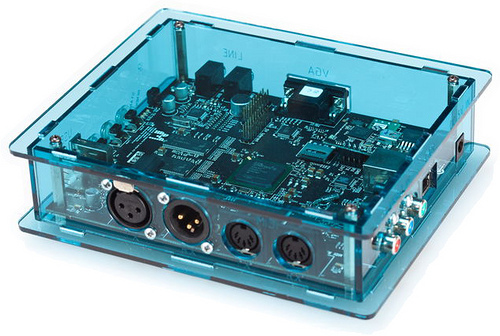
\includegraphics[scale=1]{milky_board.jpg}
\caption{Photo de la Milkymist One}
\label{milky-board}
\end{figure}

\subsubsection{Le firmware}

Le système d'exploitation qui s'exécute sur la \textit{Milkymist One} est une distribution linux appelée \textit{uClinux} qui a été adapté en même temps que la carte. Cette version de linux fonctionne sur des processeurs dédiés aux systèmes temps réel, c'est-à-dire des systèmes qui n'ont pas de MMU (\english{Memory Management Unit}) et qui ne gère pas de mécanismes de protection de la mémoire. Ce système d'exploitation a déjà été porté sur des microcontrôleurs comme certains 8-bits fabriqués par \brand{Atmel} ou d'autres PIC de chez \brand{Microchip}.\\
Le système complet se compose d'un BIOS écrit en ROM qui charge le noyau par le biais d'internet ou de la carte SD et de toutes les applications de traitement multimédia.\\

La carte dont dispose l'INSA, la \brand{Digilent} \nexys{} (figure \ref{nexys3-board}), comprend également une Spartan6 ainsi qu'un bloc de 16 MB de RAM, une interface de sortie VGA, un connecteur USB et un port Ethernet.

\begin{figure}[h!]
\centering
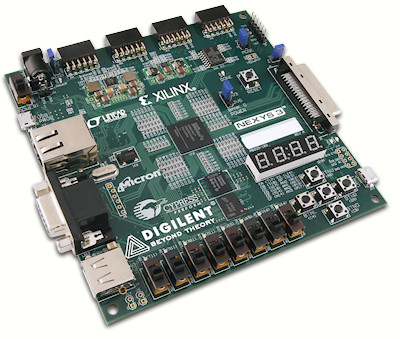
\includegraphics[scale=0.5]{nexys3.jpg}
\caption{Photo de la \nexys{} distribuée par \brand{Digilent}}
\label{nexys3-board}
\end{figure}
